\section{Introduction}
\label{sec:introduction}
A retrieval service places a user's question and conversation history ahead of a long, mostly immutable document collection. Another authorized tenant asks a different question over the same documents. The stable context is reusable at the application level, but native prefix caching stops matching at the first changed token; it cannot recover the documents' downstream KV. This ordering is not hypothetical: a fixed revision of an Azure RAG demonstration places history and question before retrieved sources~\cite{azuretemplate}. Our measured task-preserving traces likewise have 98.36--98.52\% stable-body tokens, yet recover only 0.030--0.034\% of that stable body through native prefix hits (Section~\ref{sec:background}).

An obvious remedy is to move stable documents before the changing fields. That does not make the result deployable. \emph{First}, the reorder must preserve data, causal and positional dependencies. \emph{Second}, a dependency-valid reorder can still change an autoregressive answer, so a legal layout needs behavioral evidence before use. \emph{Third}, a speculative candidate can become visible in the shared cache before qualification completes, and an otherwise valid reuse may cross a stale template or unauthorized scope. A cache hit, a behaviorally admissible layout and a published shared block are three different facts.

Prior mechanisms solve important but different parts of this problem. PagedAttention and RadixAttention implement exact-prefix reuse~\cite{vllm2023,sglang2024}; Prompt Cache provides reusable schemas~\cite{promptcache2024}; CacheBlend and EPIC explore cross-position execution~\cite{cacheblend2025,epic2025}. Application-aware scheduling and relational row/field reordering expose further reuse opportunities~\cite{parrot2024,llmqueries2025}. ContractKV addresses the complementary service decision: binding transformed state to applicable behavioral evidence, authorized consumers and an atomic publication boundary (Section~\ref{sec:background}).

\noindent\textbf{Our claim.} \emph{A structurally reusable KV prefix becomes a useful multi-tenant service object when legal compilation, execution-scoped behavioral admission, transactional publication and authorized qualification amortization are governed together.} We realize this service object through four coupled mechanisms: legal compilation, scoped admission, transactional publication and template-level qualification sharing. Figure~\ref{fig:architecture} follows an example request from raw order to an admitted, physically shared prefix.

\begin{figure*}[t]
\centering
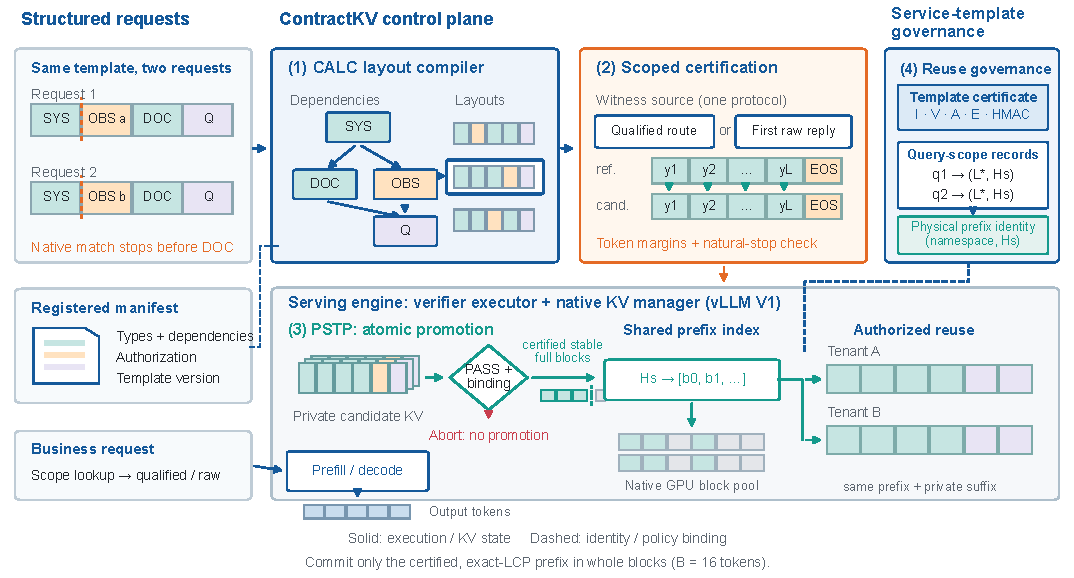
\includegraphics[width=\textwidth]{figures/fig1_architecture.pdf}
\caption{ContractKV makes a compiled stable prefix an evidence-bound service object. CALC repairs a structural prefix gap; the evaluated witness protocols supply scoped token-path evidence; PSTP commits eligible state only after PASS and a valid binding. Authorized tenants of the same template share the prefix and keep changing suffixes private. Template certificates and client query records associate applicable qualifications with the physical prefix (Table~\ref{tab:qualification-protocols}). The commit cut excludes incomplete blocks and private suffixes.}
\label{fig:architecture}
\end{figure*}

Our contributions connect each mechanism to a measurable service property:
\begin{enumerate}
\item \textbf{CALC: dependency-aware prefix compilation.} CALC constructs legal stable-prefix layouts and derives their identities after full-prompt retokenization, exposing reuse opportunities that native contiguous matching cannot reach (Sections~\ref{sec:calc} and~\ref{sec:mainresults}).
\item \textbf{Scoped behavioral certification.} Token-path and termination evidence binds a candidate to its declared execution scope. Free-running task pairs measure behavior preservation, and controlled candidate challenges establish the value of admission over layout alone (Sections~\ref{sec:scope} and~\ref{sec:quality}).
\item \textbf{PSTP: transactional shared-state publication.} The engine keeps candidate KV private until PASS and publishes only certified exact-prefix full blocks. Rejection, interruption and binding failure preserve the shared publication boundary (Sections~\ref{sec:pstp} and~\ref{sec:ablation}).
\item \textbf{Service-Template Certificates.} A versioned, authorization-bound service object lets tenants share a qualified physical prefix and its evidence cost. Fixed-layout controls isolate qualification amortization, while arrival and density studies measure its service value (Sections~\ref{sec:template} and~\ref{sec:deployment}).
\end{enumerate}

Task-preserving zero-slack serving achieves 1.619$\times$/1.109$\times$/1.070$\times$ complete-service throughput on Qwen/Mistral/Llama, retaining raw output IDs in all 1,296 admitted future pairs. Deployment-template controls reduce verifier calls 25-fold and unhidden exposure 7.7-fold; an 80\%-load point gains 0.658 SLO-compliant requests/s. Table~\ref{tab:qualification-protocols} defines the witness, scope and cost unit of each protocol. These results show how \emph{admission, publication and qualification sharing turn a reuse opportunity into a service asset}.
